See Fig. 	\ref{fig:4.2.4_circle}.  The  general equation for the circle can be given as
\begin{align}
\vec{x}^T\vec{x} + 2\vec{O}^T\vec{x} +\norm{O}^2 - \vec{r}^2 &= 0
\end{align}
given equation of circle
\begin{align}
\vec{x}^T\vec{x} -25&= 0
\end{align} 
comparing bothe of equation we can find the value of r and value of  $\vec{O}$
\begin{align}
\vec{r}&= 4
\\
\vec{O} &= \myvec{0\\0}
\\
\implies \vec{B}-\vec{O} &= \myvec{-2.5\\3.5}
\\
\implies \norm{\vec{B} - \vec{O}}^2 &= 18.5 < 25
\\
\text{or, } OB < r&
\end{align} 
Hence, $\vec{B}$ lies inside the circle.

The following code plots Fig. 	\ref{fig:4.2.4_circle}

	\begin{lstlisting}
solutions/4/codes/circle/circle2.py
	\end{lstlisting}
\begin{figure}[!ht]
	\centering
	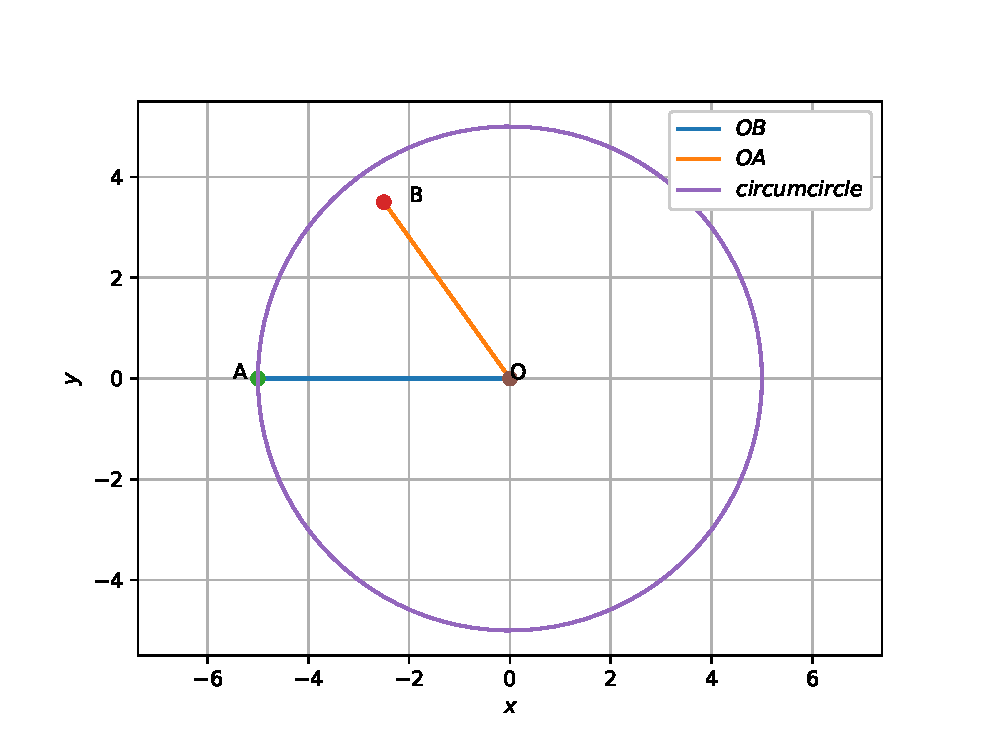
\includegraphics[width=\columnwidth]{./solutions/4/figures/circle/circle2.eps}
	\caption{circle }
	\label{fig:4.2.4_circle}
\end{figure}
